\documentclass[11pt]{a0poster}

\usepackage{url}
\usepackage{graphicx}
\usepackage[usenames,dvipsnames]{color}
\usepackage[margin=0in]{geometry}
\usepackage{xcolor}
\usepackage{graphicx}
\usepackage{amsmath}

\widowpenalty=500
\clubpenalty=500
\fboxsep=0pt

\renewcommand*{\familydefault}{\sfdefault}

\date{}

\begin{document}

\begin{minipage}{0.887\linewidth}
\vspace{130pt}
\hspace{92pt}
\color{Blue}
{\fontsize{3cm}{1em} \textbf{Analyzing Large Scale Genotype Datasets With Gnocchi}}

%\vspace{0pt}
\hspace{92pt}
\huge Frank~Austin~Nothaft, fnothaft@berkeley.edu

\vspace{130pt}
\end{minipage}
\begin{minipage}{0.113\linewidth}

\includegraphics[scale=0.6]{ucseal_540_139.pdf}
\end{minipage}

{\color{Blue}\noindent\makebox[\linewidth]{\rule{\paperwidth}{30pt}}}

\noindent\colorbox{Yellow}{
\begin{minipage}[t][2045pt][t]{\linewidth}

\noindent\begin{minipage}{0.025\linewidth}
\hfill
\pagebreak
\end{minipage}
\begin{minipage}{0.3\linewidth}
\vspace{75pt}
\colorbox{Blue}{
\begin{minipage}{\linewidth}
\vspace{25pt}
\begin{center}
\Huge \bf \color{White} Background
\end{center}
\vspace{10pt}
\end{minipage}
}
\colorbox{White}{
\begin{minipage}[t][700pt][t]{\linewidth}
\color{Blue}
\vspace{20pt}
\LARGE
Although the ADAM project defines parallel APIs for processing large genomic
datasets, these APIs are mostly designed for running ETL jobs against read
data. While some of these APIs can be reused for variant data, genomic variants
can benefit from different APIs:

\vspace{33pt}
\begin{itemize}
\item Variant datasets need to be analyzed in the context of a population.
\item Genotype datasets have a natural mapping to matrix-like structures.
\end{itemize}
\vspace{33pt}

In Gnocchi, we introduce a variety of APIs for running matrix-like calculations
against large, genomic variant datasets.
\hfill
\pagebreak
\end{minipage}
}

\vspace{75pt}
\colorbox{Blue}{
\begin{minipage}{\linewidth}
\vspace{25pt}
\begin{center}
\Huge \bf \color{White} Performance
\end{center}
\vspace{10pt}
\end{minipage}
}
\colorbox{White}{
\begin{minipage}[t][920pt][t]{\linewidth}
\color{Blue}
\vspace{20pt}
\LARGE
\begin{itemize}
\item Evaluated for speedup on 1,024 core cluster
\item Run against NCI-60 cell line dataset + phenotypes
\item 16GB of memory per core, 0.75TB HDD, 10G interconnect
\end{itemize}
\begin{center}
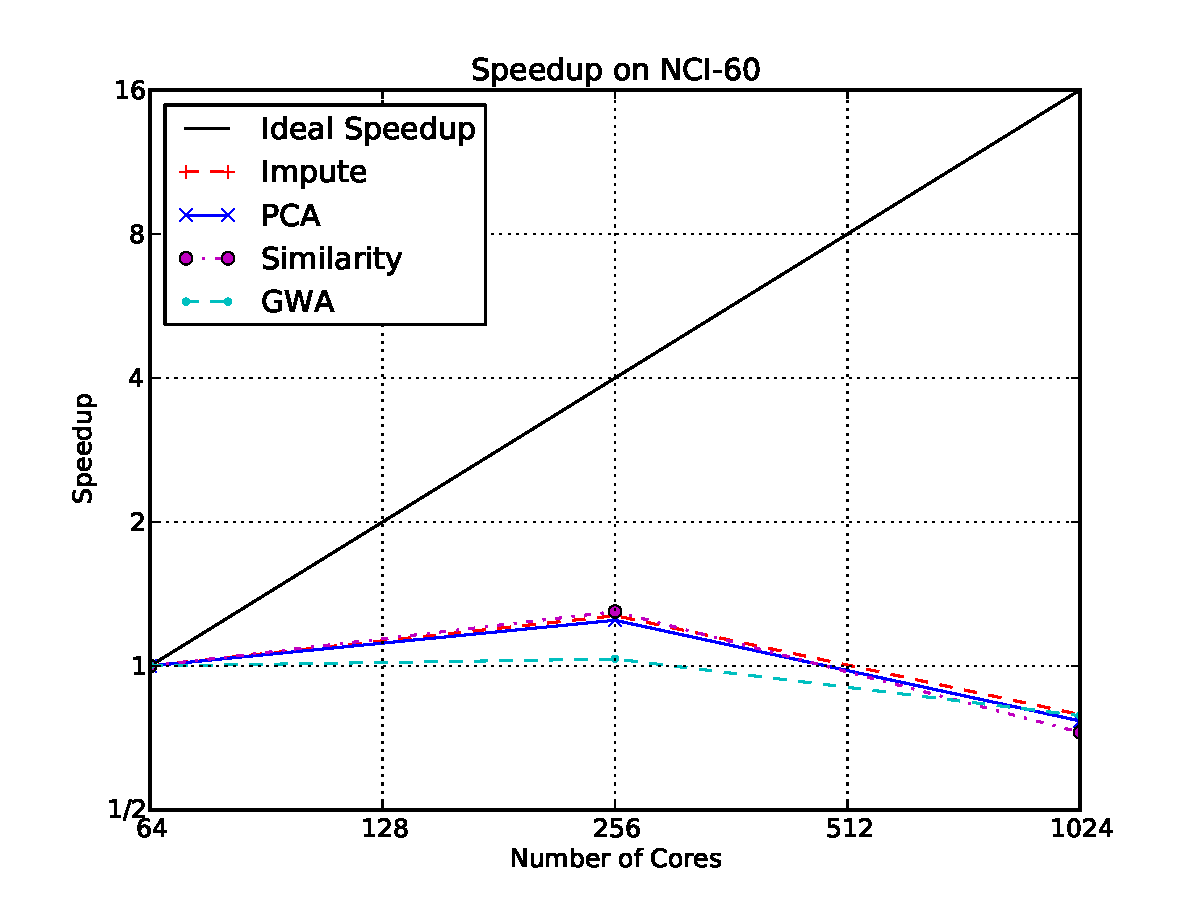
\includegraphics[width=0.95\linewidth]{graphs/speedup.pdf}
\end{center}
\pagebreak
\end{minipage}
}
\pagebreak
\end{minipage}
\begin{minipage}{0.03\linewidth}
\hfill
\pagebreak
\end{minipage}
\begin{minipage}{0.6\linewidth}

\vspace{70pt}
\colorbox{Blue}{
\begin{minipage}[t]{\linewidth}
\vspace{30pt}
\begin{center}
\Huge \bf \color{White} Architecture
\end{center}
\vspace{17pt}
\end{minipage}
}
\colorbox{White}{
\begin{minipage}[t][1170pt][t]{\linewidth}
\begin{minipage}{0.01\linewidth}
\hfill
\pagebreak
\end{minipage}
\begin{minipage}{0.48\linewidth}
\vspace{-25pt}
\color{Blue}
\begin{center}
\huge Matrix methods:
\end{center}
\LARGE
Traditionally, genomic variant storage formats have stored genotypes as
``row''-oriented data. In this representation, all of the genotypes for a
single variant are stored in a single record. While this makes matrix
calculations straightforward, it limits scalability, as the size of a
single record grows with the number of individuals we are looking at.

\vspace{20pt}

ADAM uses a ``cell'' oriented approach, where genotypes belong
to independent records. As such, we must be able to reconstruct genotype
matrices. We do this by running a \texttt{groupBy} on each position.

\vspace{20pt}

Frequently, people want to run PCA on genotype matrices, however, this
is difficult to do in Spark because genotype matrices are flat and wide.
Instead, we transpose the genotype matrix and compute PCA via the SVD:

\vspace{-40pt}
\begin{center}
$$
A = U \Sigma V^{\text{T}}
$$
$$
A^{\text{T}} = V \Sigma U^{\text{T}}
$$
$$
T_A = U \Sigma
$$
\end{center}
\end{minipage}
\begin{minipage}{0.01\linewidth}
\hfill
\pagebreak
\end{minipage}
\begin{minipage}{0.48\linewidth}
\vspace{30pt}
\hspace{100pt}
\color{Blue}
\vspace{-50pt}
\begin{center}
\huge Aggregation queries:
\end{center}
\LARGE
While matrices are used to run many machine learning kernels that are used to
identify population structure, not all algorithms map to matrices. Another
common pattern is per-variant aggregation:

\vspace{20pt}

\begin{center}
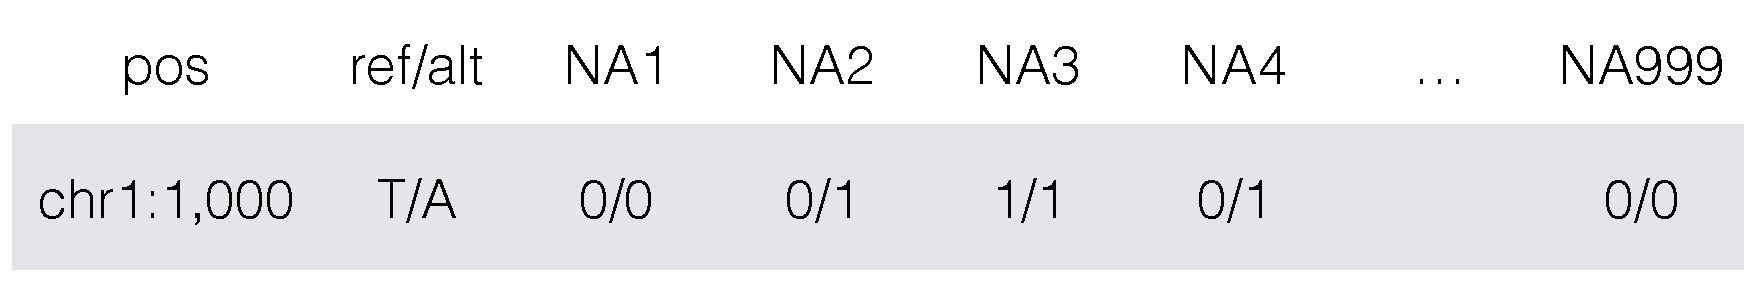
\includegraphics[width=0.95\linewidth]{aggregation.pdf}

\vspace{-40pt}

$$
a_0 = f(i, g_0)
$$
$$
a_i = f(a_{i-1}, g_i), \forall i \in [1, N)
$$

\end{center}

\vspace{40pt}

We use this pattern to implement a case-control genome wide association
study~(GWAS) test. This kernel applies a $\chi^2$ test to the cross-join of
all genotypes and phenotypes for a population to test for the association of
a phenotype with an individual variant.

\vspace{20pt}

This pattern is typically used to iteratively train models, such as a linear
regression at each variant, as well as to compute per-site statistics.
\end{minipage}
\pagebreak
\end{minipage}
}

\vspace{75pt}
\begin{minipage}{\linewidth}
\colorbox{Blue}{
\begin{minipage}[t]{\linewidth}
\vspace{30pt}
\begin{center}
\Huge \bf \color{White} Future Work
\end{center}
\vspace{17pt}
\end{minipage}
}
\colorbox{White}{
\begin{minipage}[t][420pt][t]{\linewidth}
\begin{minipage}{0.005\linewidth}
\hfill
\pagebreak
\end{minipage}
\begin{minipage}{0.98\linewidth}
\LARGE
\vspace{10pt}
\color{Blue}
\begin{itemize}
\item Many of these stages operate on a matrix of genotypes. Currently, we build
this matrix from the input genotypes each time via a groupBy.
\begin{itemize}
\item In practice, we frequently work on a sparse representation of the matrix,
which is much smaller than the full matrix. We can materialize this.
\item Additionally, the groupBy cost can be minimized through better partitioning
strategies (e.g., coordinate sort).
\end{itemize}
\item We are working on more clustering variants (e.g., K-means) and regression
tests.
\item Additionally, the regression kernels expose interesting join patterns.
\end{itemize}
\end{minipage}
\end{minipage}
}
\end{minipage}
\end{minipage}
\end{minipage}
}

\end{document}
